\documentclass[ignorenonframetext,]{beamer}
% =====================================================================
% Shared Beamer preamble for all regression lecture slides
%
% Usage in each lecture file:
%   \documentclass[ignorenonframetext,]{beamer}
%   % =====================================================================
% Shared Beamer preamble for all regression lecture slides
%
% Usage in each lecture file:
%   \documentclass[ignorenonframetext,]{beamer}
%   % =====================================================================
% Shared Beamer preamble for all regression lecture slides
%
% Usage in each lecture file:
%   \documentclass[ignorenonframetext,]{beamer}
%   \input{preamble}
%   \title{...}
%   \begin{document}
%   \frame{\titlepage}
%   ...
% =====================================================================

% ---------------------------------------------------------------------
% Theme and captions
% ---------------------------------------------------------------------
\setbeamertemplate{caption}[numbered]
\setbeamertemplate{caption label separator}{: }
\setbeamercolor{caption name}{fg=normal text.fg}
\beamertemplatenavigationsymbolsempty

% ---------------------------------------------------------------------
% Fonts and encoding (pdfLaTeX, XeLaTeX and LuaLaTeX all supported)
% ---------------------------------------------------------------------
\usepackage{lmodern}
\usepackage{amssymb,amsmath}
\usepackage{ifxetex,ifluatex}
\ifnum 0\ifxetex 1\fi\ifluatex 1\fi=0 % if pdftex
\usepackage[T1]{fontenc}
\usepackage[utf8]{inputenc}
\else % if luatex or xelatex
\ifxetex
\usepackage{mathspec}
\else
\usepackage{fontspec}
\fi
\defaultfontfeatures{Ligatures=TeX,Scale=MatchLowercase}
\fi

\usetheme{Madrid}
\usecolortheme{orchid}
\usepackage{beamerthemesplit}

% use upquote if available, for straight quotes in verbatim environments
\IfFileExists{upquote.sty}{\usepackage{upquote}}{}
% use microtype if available
\IfFileExists{microtype.sty}{%
\usepackage{microtype}
\UseMicrotypeSet[protrusion]{basicmath} % disable protrusion for tt fonts
}{}

% ---------------------------------------------------------------------
% Packages
% ---------------------------------------------------------------------
\usepackage{amsthm}
\usepackage{bm}
\usepackage{bbm, dsfont}
\usepackage{extarrows}
\usepackage{kotex}
\usepackage{natbib}
\usepackage{graphicx}
\usepackage{booktabs}
\usepackage{multirow}
\usepackage{makecell}
\usepackage{array}
\usepackage{arydshln}
\usepackage{hhline}
\usepackage{caption}
\usepackage{comment}
\usepackage{needspace}
\usepackage{listings}
\usepackage{tikz}
\usetikzlibrary{arrows,shapes,calc,positioning}

\newif\ifbibliography

% ---------------------------------------------------------------------
% Graphics: scale images so that they do not overflow the page margins
% by default; explicit \includegraphics options still take precedence.
% ---------------------------------------------------------------------
\makeatletter
\def\maxwidth{\ifdim\Gin@nat@width>\linewidth\linewidth\else\Gin@nat@width\fi}
\def\maxheight{\ifdim\Gin@nat@height>\textheight0.8\textheight\else\Gin@nat@height\fi}
\makeatother
\setkeys{Gin}{width=\maxwidth,height=\maxheight,keepaspectratio}

% ---------------------------------------------------------------------
% Colors
% ---------------------------------------------------------------------
\definecolor{azure}{rgb}{0, 0.4, 0.8}
\definecolor{crimson}{rgb}{0.8, 0.4, 0}
\definecolor{gold}{rgb}{0.72, 0.53, 0.04}
\definecolor{ciel}{rgb}{0.39, 0.58, 0.93}
\definecolor{dgreen}{rgb}{0.01, 0.75, 0.24}

% ---------------------------------------------------------------------
% Layout
% ---------------------------------------------------------------------
% Prevent slide breaks in the middle of a paragraph:
\widowpenalties 1 10000
\raggedbottom

\setlength{\parindent}{0pt}
\setlength{\parskip}{6pt plus 2pt minus 1pt}
\setlength{\emergencystretch}{3em}  % prevent overfull lines
\providecommand{\tightlist}{%
\setlength{\itemsep}{0pt}\setlength{\parskip}{0pt}}
\setcounter{secnumdepth}{0}
\captionsetup[table]{belowskip=0pt,aboveskip=0pt}
\captionsetup[figure]{belowskip=0pt,aboveskip=0pt}

% ---------------------------------------------------------------------
% Theorem-like environments
% (Beamer already provides theorem, corollary, lemma, definition,
%  example, ... ; the short names below are used by the lecture files.)
% ---------------------------------------------------------------------
\theoremstyle{plain}
\newtheorem{thm}{Theorem}[section]
\newtheorem{cor}[thm]{Corollary}
\newtheorem{lem}[thm]{Lemma}
\newtheorem{prop}[thm]{Proposition}
\theoremstyle{definition}
\newtheorem{defn}{Definition}[section]
\newtheorem{remk}{Remark}[section]
\newtheorem{exam}{Example}[section]
\newtheorem{prob}{Exercise}[section]
\newtheorem{solu2}{Solution}[section]
\newtheorem{model}{Model}

% ---------------------------------------------------------------------
% Macros
% ---------------------------------------------------------------------
\newcommand{\E}[1]{{\mathbb E}\left[#1\right]}
\newcommand{\Var}[1]{{\mathrm Var}\left(#1\right)}
\newcommand{\var}{\operatorname{Var}}
\newcommand{\dif}{\operatorname{d}}
\newcommand{\parallelsum}{\mathbin{\!/\mkern-5mu/\!}}
\newcommand\tab[1][1cm]{\hspace*{#1}}
\newcommand{\brtexttt}[1]{\texttt{\color{brown}{#1}}}

% ---------------------------------------------------------------------
% Author and date (common to all lectures)
% ---------------------------------------------------------------------
\author[Himchan Jeong]{\large{Himchan Jeong, PhD, FSA}}
\date{}

%   \title{...}
%   \begin{document}
%   \frame{\titlepage}
%   ...
% =====================================================================

% ---------------------------------------------------------------------
% Theme and captions
% ---------------------------------------------------------------------
\setbeamertemplate{caption}[numbered]
\setbeamertemplate{caption label separator}{: }
\setbeamercolor{caption name}{fg=normal text.fg}
\beamertemplatenavigationsymbolsempty

% ---------------------------------------------------------------------
% Fonts and encoding (pdfLaTeX, XeLaTeX and LuaLaTeX all supported)
% ---------------------------------------------------------------------
\usepackage{lmodern}
\usepackage{amssymb,amsmath}
\usepackage{ifxetex,ifluatex}
\ifnum 0\ifxetex 1\fi\ifluatex 1\fi=0 % if pdftex
\usepackage[T1]{fontenc}
\usepackage[utf8]{inputenc}
\else % if luatex or xelatex
\ifxetex
\usepackage{mathspec}
\else
\usepackage{fontspec}
\fi
\defaultfontfeatures{Ligatures=TeX,Scale=MatchLowercase}
\fi

\usetheme{Madrid}
\usecolortheme{orchid}
\usepackage{beamerthemesplit}

% use upquote if available, for straight quotes in verbatim environments
\IfFileExists{upquote.sty}{\usepackage{upquote}}{}
% use microtype if available
\IfFileExists{microtype.sty}{%
\usepackage{microtype}
\UseMicrotypeSet[protrusion]{basicmath} % disable protrusion for tt fonts
}{}

% ---------------------------------------------------------------------
% Packages
% ---------------------------------------------------------------------
\usepackage{amsthm}
\usepackage{bm}
\usepackage{bbm, dsfont}
\usepackage{extarrows}
\usepackage{kotex}
\usepackage{natbib}
\usepackage{graphicx}
\usepackage{booktabs}
\usepackage{multirow}
\usepackage{makecell}
\usepackage{array}
\usepackage{arydshln}
\usepackage{hhline}
\usepackage{caption}
\usepackage{comment}
\usepackage{needspace}
\usepackage{listings}
\usepackage{tikz}
\usetikzlibrary{arrows,shapes,calc,positioning}

\newif\ifbibliography

% ---------------------------------------------------------------------
% Graphics: scale images so that they do not overflow the page margins
% by default; explicit \includegraphics options still take precedence.
% ---------------------------------------------------------------------
\makeatletter
\def\maxwidth{\ifdim\Gin@nat@width>\linewidth\linewidth\else\Gin@nat@width\fi}
\def\maxheight{\ifdim\Gin@nat@height>\textheight0.8\textheight\else\Gin@nat@height\fi}
\makeatother
\setkeys{Gin}{width=\maxwidth,height=\maxheight,keepaspectratio}

% ---------------------------------------------------------------------
% Colors
% ---------------------------------------------------------------------
\definecolor{azure}{rgb}{0, 0.4, 0.8}
\definecolor{crimson}{rgb}{0.8, 0.4, 0}
\definecolor{gold}{rgb}{0.72, 0.53, 0.04}
\definecolor{ciel}{rgb}{0.39, 0.58, 0.93}
\definecolor{dgreen}{rgb}{0.01, 0.75, 0.24}

% ---------------------------------------------------------------------
% Layout
% ---------------------------------------------------------------------
% Prevent slide breaks in the middle of a paragraph:
\widowpenalties 1 10000
\raggedbottom

\setlength{\parindent}{0pt}
\setlength{\parskip}{6pt plus 2pt minus 1pt}
\setlength{\emergencystretch}{3em}  % prevent overfull lines
\providecommand{\tightlist}{%
\setlength{\itemsep}{0pt}\setlength{\parskip}{0pt}}
\setcounter{secnumdepth}{0}
\captionsetup[table]{belowskip=0pt,aboveskip=0pt}
\captionsetup[figure]{belowskip=0pt,aboveskip=0pt}

% ---------------------------------------------------------------------
% Theorem-like environments
% (Beamer already provides theorem, corollary, lemma, definition,
%  example, ... ; the short names below are used by the lecture files.)
% ---------------------------------------------------------------------
\theoremstyle{plain}
\newtheorem{thm}{Theorem}[section]
\newtheorem{cor}[thm]{Corollary}
\newtheorem{lem}[thm]{Lemma}
\newtheorem{prop}[thm]{Proposition}
\theoremstyle{definition}
\newtheorem{defn}{Definition}[section]
\newtheorem{remk}{Remark}[section]
\newtheorem{exam}{Example}[section]
\newtheorem{prob}{Exercise}[section]
\newtheorem{solu2}{Solution}[section]
\newtheorem{model}{Model}

% ---------------------------------------------------------------------
% Macros
% ---------------------------------------------------------------------
\newcommand{\E}[1]{{\mathbb E}\left[#1\right]}
\newcommand{\Var}[1]{{\mathrm Var}\left(#1\right)}
\newcommand{\var}{\operatorname{Var}}
\newcommand{\dif}{\operatorname{d}}
\newcommand{\parallelsum}{\mathbin{\!/\mkern-5mu/\!}}
\newcommand\tab[1][1cm]{\hspace*{#1}}
\newcommand{\brtexttt}[1]{\texttt{\color{brown}{#1}}}

% ---------------------------------------------------------------------
% Author and date (common to all lectures)
% ---------------------------------------------------------------------
\author[Himchan Jeong]{\large{Himchan Jeong, PhD, FSA}}
\date{}

%   \title{...}
%   \begin{document}
%   \frame{\titlepage}
%   ...
% =====================================================================

% ---------------------------------------------------------------------
% Theme and captions
% ---------------------------------------------------------------------
\setbeamertemplate{caption}[numbered]
\setbeamertemplate{caption label separator}{: }
\setbeamercolor{caption name}{fg=normal text.fg}
\beamertemplatenavigationsymbolsempty

% ---------------------------------------------------------------------
% Fonts and encoding (pdfLaTeX, XeLaTeX and LuaLaTeX all supported)
% ---------------------------------------------------------------------
\usepackage{lmodern}
\usepackage{amssymb,amsmath}
\usepackage{ifxetex,ifluatex}
\ifnum 0\ifxetex 1\fi\ifluatex 1\fi=0 % if pdftex
\usepackage[T1]{fontenc}
\usepackage[utf8]{inputenc}
\else % if luatex or xelatex
\ifxetex
\usepackage{mathspec}
\else
\usepackage{fontspec}
\fi
\defaultfontfeatures{Ligatures=TeX,Scale=MatchLowercase}
\fi

\usetheme{Madrid}
\usecolortheme{orchid}
\usepackage{beamerthemesplit}

% use upquote if available, for straight quotes in verbatim environments
\IfFileExists{upquote.sty}{\usepackage{upquote}}{}
% use microtype if available
\IfFileExists{microtype.sty}{%
\usepackage{microtype}
\UseMicrotypeSet[protrusion]{basicmath} % disable protrusion for tt fonts
}{}

% ---------------------------------------------------------------------
% Packages
% ---------------------------------------------------------------------
\usepackage{amsthm}
\usepackage{bm}
\usepackage{bbm, dsfont}
\usepackage{extarrows}
\usepackage{kotex}
\usepackage{natbib}
\usepackage{graphicx}
\usepackage{booktabs}
\usepackage{multirow}
\usepackage{makecell}
\usepackage{array}
\usepackage{arydshln}
\usepackage{hhline}
\usepackage{caption}
\usepackage{comment}
\usepackage{needspace}
\usepackage{listings}
\usepackage{tikz}
\usetikzlibrary{arrows,shapes,calc,positioning}

\newif\ifbibliography

% ---------------------------------------------------------------------
% Graphics: scale images so that they do not overflow the page margins
% by default; explicit \includegraphics options still take precedence.
% ---------------------------------------------------------------------
\makeatletter
\def\maxwidth{\ifdim\Gin@nat@width>\linewidth\linewidth\else\Gin@nat@width\fi}
\def\maxheight{\ifdim\Gin@nat@height>\textheight0.8\textheight\else\Gin@nat@height\fi}
\makeatother
\setkeys{Gin}{width=\maxwidth,height=\maxheight,keepaspectratio}

% ---------------------------------------------------------------------
% Colors
% ---------------------------------------------------------------------
\definecolor{azure}{rgb}{0, 0.4, 0.8}
\definecolor{crimson}{rgb}{0.8, 0.4, 0}
\definecolor{gold}{rgb}{0.72, 0.53, 0.04}
\definecolor{ciel}{rgb}{0.39, 0.58, 0.93}
\definecolor{dgreen}{rgb}{0.01, 0.75, 0.24}

% ---------------------------------------------------------------------
% Layout
% ---------------------------------------------------------------------
% Prevent slide breaks in the middle of a paragraph:
\widowpenalties 1 10000
\raggedbottom

\setlength{\parindent}{0pt}
\setlength{\parskip}{6pt plus 2pt minus 1pt}
\setlength{\emergencystretch}{3em}  % prevent overfull lines
\providecommand{\tightlist}{%
\setlength{\itemsep}{0pt}\setlength{\parskip}{0pt}}
\setcounter{secnumdepth}{0}
\captionsetup[table]{belowskip=0pt,aboveskip=0pt}
\captionsetup[figure]{belowskip=0pt,aboveskip=0pt}

% ---------------------------------------------------------------------
% Theorem-like environments
% (Beamer already provides theorem, corollary, lemma, definition,
%  example, ... ; the short names below are used by the lecture files.)
% ---------------------------------------------------------------------
\theoremstyle{plain}
\newtheorem{thm}{Theorem}[section]
\newtheorem{cor}[thm]{Corollary}
\newtheorem{lem}[thm]{Lemma}
\newtheorem{prop}[thm]{Proposition}
\theoremstyle{definition}
\newtheorem{defn}{Definition}[section]
\newtheorem{remk}{Remark}[section]
\newtheorem{exam}{Example}[section]
\newtheorem{prob}{Exercise}[section]
\newtheorem{solu2}{Solution}[section]
\newtheorem{model}{Model}

% ---------------------------------------------------------------------
% Macros
% ---------------------------------------------------------------------
\newcommand{\E}[1]{{\mathbb E}\left[#1\right]}
\newcommand{\Var}[1]{{\mathrm Var}\left(#1\right)}
\newcommand{\var}{\operatorname{Var}}
\newcommand{\dif}{\operatorname{d}}
\newcommand{\parallelsum}{\mathbin{\!/\mkern-5mu/\!}}
\newcommand\tab[1][1cm]{\hspace*{#1}}
\newcommand{\brtexttt}[1]{\texttt{\color{brown}{#1}}}

% ---------------------------------------------------------------------
% Author and date (common to all lectures)
% ---------------------------------------------------------------------
\author[Himchan Jeong]{\large{Himchan Jeong, PhD, FSA}}
\date{}


\title{Variable Selection in Linear Models}
\subtitle{Subset Selection, Shrinkage Methods, Model Evaluation}

\begin{document}
\frame{\titlepage}

% ---------------------------------------------------------------------
\begin{frame}{Agenda}
\begin{enumerate}
	\item \textbf{Why Variable Selection?}\\
	{\small\emph{The problem with RSS/$R^2$ for model selection}}
	\item \textbf{Subset Selection}\\
	{\small\emph{Best subset, forward, backward \& hybrid}}
	\item \textbf{Choosing the Best Model}\\
	{\small\emph{$C_p$, AIC, BIC, Adjusted $R^2$, Cross-Validation}}
	\item \textbf{Shrinkage Methods}\\
	{\small\emph{Ridge Regression \& The Lasso}}
	\item \textbf{Tuning Parameter Selection}\\
	{\small\emph{Cross-validation for $\lambda$}}
\end{enumerate}

\vfill
{\footnotesize\emph{Based on: An Introduction to Statistical Learning (Chapter 6)}}
\end{frame}

% ---------------------------------------------------------------------
\begin{frame}{Why Variable Selection?}
\begin{columns}[T]
\begin{column}{0.49\textwidth}
\begin{alertblock}{The Problem}
\small
\textbf{Including too many predictors hurts model quality:}
\begin{itemize}
	\item RSS always decreases as predictors are added
	\item $R^2$ always increases with more variables
	\item Training error $\neq$ Test error
	\item Overfitting leads to high variance
	\item Hard to interpret large models
\end{itemize}
\end{alertblock}
\end{column}
\begin{column}{0.49\textwidth}
\begin{exampleblock}{Goals of Variable Selection}
\small
\textbf{Find a subset of predictors that:}
\begin{itemize}
	\item Minimizes test (not training) error
	\item Reduces model complexity
	\item Improves interpretability
	\item Reduces variance at cost of small bias
	\item Selects signal variables, removes noise
\end{itemize}
\end{exampleblock}
\end{column}
\end{columns}
\end{frame}

% ---------------------------------------------------------------------
\begin{frame}{Three Approaches to Variable Selection}
\begin{columns}[T]
\begin{column}{0.32\textwidth}
\begin{block}{\small Subset Selection}
\footnotesize
\begin{itemize}
	\item Best Subset
	\item Forward Stepwise
	\item Backward Stepwise
	\item Hybrid Methods
\end{itemize}
\end{block}
\end{column}
\begin{column}{0.32\textwidth}
\begin{block}{\small Shrinkage Methods}
\footnotesize
\begin{itemize}
	\item Ridge Regression
	\item The Lasso
	\item Shrink coefficients $\rightarrow 0$
	\item Retain all predictors (Ridge)
\end{itemize}
\end{block}
\end{column}
\begin{column}{0.32\textwidth}
\begin{block}{\small Dimension Reduction}
\footnotesize
\begin{itemize}
	\item Principal Components
	\item Partial Least Squares
	\item Project to subspace
	\item (Beyond this chapter)
\end{itemize}
\end{block}
\end{column}
\end{columns}

\vspace{12pt}
\centering
{\small\emph{Focus of this presentation: Subset Selection + Shrinkage Methods}}
\end{frame}

% =====================================================================
\section{Part 1: Subset Selection}

\begin{frame}
\centering
{\Large\usebeamercolor[fg]{structure}\textbf{Part 1: Subset Selection}}

\vspace{12pt}
Choosing the right predictors from $2^p$ possible models
\end{frame}

% ---------------------------------------------------------------------
\begin{frame}{Best Subset Selection}
\emph{Fit a separate least squares regression for every possible combination of predictors.}

\small
\begin{tabular}{@{}p{0.13\textwidth}p{0.82\textwidth}@{}}
\toprule
\textbf{Step 1} & \textbf{Null Model $\mathcal{M}_0$}\\
& Model with no predictors --- predicts sample mean for every observation.\\
\midrule
\textbf{Step 2} & \textbf{Fit All Size-$k$ Models}\\
& For $k = 1, 2, \ldots, p$: fit all $\binom{p}{k}$ models with exactly $k$ predictors.\\
& Pick the best $\mathcal{M}_k$ = smallest RSS (or largest $R^2$).\\
\midrule
\textbf{Step 3} & \textbf{Select Single Best Model}\\
& Choose from $\mathcal{M}_0, \mathcal{M}_1, \ldots, \mathcal{M}_p$ using: Validation Error, $C_p$ (AIC), BIC, or Adjusted $R^2$.\\
\bottomrule
\end{tabular}

\vspace{6pt}
\begin{alertblock}{}
\small\textbf{Computational limit: $2^p$ models grow exponentially --- infeasible for $p > 40$}
\end{alertblock}
\end{frame}

% ---------------------------------------------------------------------
\begin{frame}{Best Subset: RSS and $R^2$ Behavior}
\begin{columns}[T]
\begin{column}{0.56\textwidth}
\centering
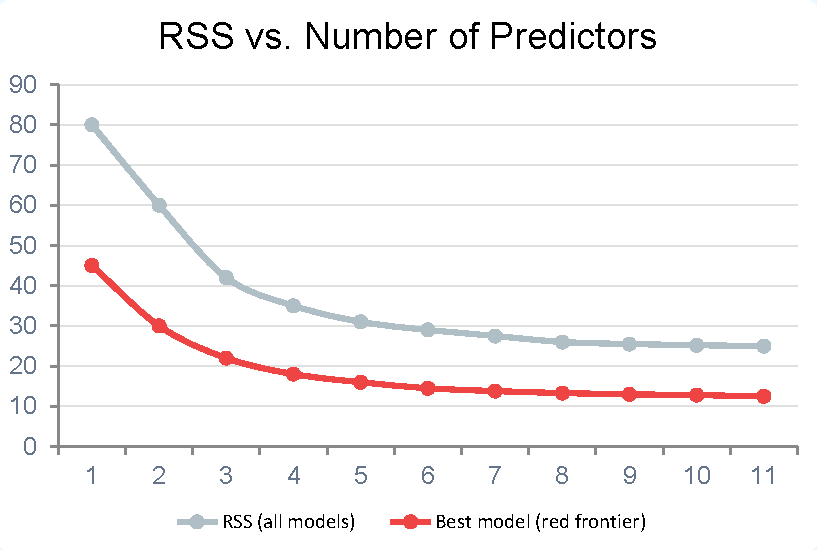
\includegraphics[width=\textwidth]{figures/varsel/varsel_rss_vs_predictors.pdf}

{\scriptsize\emph{Red frontier: best model for each size $k$}}
\end{column}
\begin{column}{0.42\textwidth}
\footnotesize
\begin{alertblock}{RSS Monotonically $\downarrow$}
Adding predictors always reduces RSS --- can't use it to pick the best model.
\end{alertblock}
\begin{block}{$R^2$ Monotonically $\uparrow$}
$R^2$ always rises with predictors --- models with all variables win trivially.
\end{block}
\begin{exampleblock}{Need Test Error}
Use validation error, $C_p$, BIC, or adjusted $R^2$ to select model size.
\end{exampleblock}
\end{column}
\end{columns}
\end{frame}

% ---------------------------------------------------------------------
\begin{frame}{Forward Stepwise Selection}
\emph{Starts with null model, adds one predictor at a time --- the one giving greatest fit improvement.}

\begin{center}

\begin{tikzpicture}[
	box/.style={draw=none, fill=blue!60!black, text=white, font=\scriptsize\bfseries,
	            align=center, minimum width=1.65cm, minimum height=0.9cm}]
	\node[box, fill=black!80] (m0) at (0,0) {$\mathcal{M}_0$\\Null model};
	\node[box] (m1) at (2.1,0) {$\mathcal{M}_1$\\Best 1-var};
	\node[box] (m2) at (4.2,0) {$\mathcal{M}_2$\\Best 2-var};
	\node[box, fill=gray] (dots) at (6.3,0) {$\ldots$};
	\node[box] (mp) at (8.4,0) {$\mathcal{M}_p$\\Full model};
	\draw[->, thick] (m0) -- (m1);
	\draw[->, thick] (m1) -- (m2);
	\draw[->, thick] (m2) -- (dots);
	\draw[->, thick] (dots) -- (mp);
\end{tikzpicture}

{\footnotesize Best model selected using: $C_p$, AIC, BIC, Adjusted $R^2$, or Cross-Validation}
\end{center}

\textbf{Computational Comparison}

\begin{center}
\small
\begin{tabular}{ccc}
\toprule
\textbf{Method} & \textbf{Models Fitted ($p=20$)} & \textbf{Works when $n < p$?}\\
\midrule
Best Subset & 1,048,576 ($2^{20}$) & No\\
Forward Stepwise & 211 & Yes $\checkmark$\\
Backward Stepwise & 211 & No\\
\bottomrule
\end{tabular}
\end{center}
\end{frame}

% ---------------------------------------------------------------------
\begin{frame}{Backward Stepwise Selection}
\emph{Starts with the full model, removes the least useful predictor one at a time.}

\footnotesize
\begin{tabular}{@{}p{0.07\textwidth}p{0.88\textwidth}@{}}
\toprule
\textbf{1} & \textbf{Start: Full Model $\mathcal{M}_p$}\\
& Begin with all $p$ predictors in the model.\\
\midrule
\textbf{2a} & \textbf{Consider Removing One}\\
& For each iteration $k = p, p-1, \ldots, 1$: consider all $k$ models that omit exactly one predictor from $\mathcal{M}_k$.\\
\midrule
\textbf{2b} & \textbf{Choose Best $\mathcal{M}_{k-1}$}\\
& Pick the model with the smallest RSS (or highest $R^2$) --- this is $\mathcal{M}_{k-1}$.\\
\midrule
\textbf{3} & \textbf{Select Final Model}\\
& Use validation error, $C_p$, BIC, or adjusted $R^2$ to choose from $\mathcal{M}_0, \mathcal{M}_1, \ldots, \mathcal{M}_p$.\\
\bottomrule
\end{tabular}

\vspace{6pt}
\begin{exampleblock}{}
\small\textbf{Key Constraint: requires $n > p$ to fit the initial full model (use Forward Stepwise when $n < p$)}
\end{exampleblock}
\end{frame}

% ---------------------------------------------------------------------
\begin{frame}{Best Subset vs. Forward Stepwise: Credit Data}
\emph{Both methods often agree --- but not always. Forward stepwise cannot revisit earlier choices.}

\begin{center}
\small
\begin{tabular}{ccc}
\toprule
\textbf{\# Variables} & \textbf{Best Subset} & \textbf{Forward Stepwise}\\
\midrule
1 & \colorbox{green!15}{rating} & \colorbox{green!15}{rating}\\
2 & \colorbox{green!15}{rating, income} & \colorbox{green!15}{rating, income}\\
3 & \colorbox{green!15}{rating, income, student} & \colorbox{green!15}{rating, income, student}\\
4 & \colorbox{red!15}{cards, income, student, limit} & \colorbox{red!15}{rating, income, student, limit}\\
\bottomrule
\end{tabular}

\vspace{4pt}
{\footnotesize \colorbox{green!15}{$\checkmark$ Match} \quad \colorbox{red!15}{$\times$ Differ}}
\end{center}

\begin{block}{}
\footnotesize
Forward stepwise keeps `rating' in the 4-variable model because $\mathcal{M}_1$ already contains it.\\
Best subset can replace it --- finding globally optimal subsets at each size.
\end{block}
\end{frame}

% ---------------------------------------------------------------------
\begin{frame}{Hybrid Approaches}
\begin{columns}[T]
\begin{column}{0.32\textwidth}
\begin{block}{\small $\rightarrow$ Forward Stepwise}
\footnotesize
Start empty, add predictors one by one. Greedy --- cannot remove what was added.
\end{block}
\end{column}
\begin{column}{0.32\textwidth}
\begin{block}{\small $\leftarrow$ Backward Stepwise}
\footnotesize
Start full, remove predictors one by one. Requires $n > p$.
\end{block}
\end{column}
\begin{column}{0.32\textwidth}
\begin{exampleblock}{\small $\leftrightarrow$ Hybrid}
\footnotesize
Add predictors sequentially BUT also remove variables that no longer improve fit after each addition.
\end{exampleblock}
\end{column}
\end{columns}

\vspace{12pt}
\small
Hybrid methods mimic best subset selection more closely while maintaining the computational efficiency of forward/backward stepwise.
\end{frame}

% =====================================================================
\section{Part 2: Choosing the Optimal Model}

\begin{frame}
\centering
{\Large\usebeamercolor[fg]{structure}\textbf{Part 2: Choosing the Optimal Model}}

\vspace{12pt}
Estimating test error to select among candidate models
\end{frame}

% ---------------------------------------------------------------------
\begin{frame}{$C_p$ and AIC Criteria}
\vspace{4pt}
{\small\emph{Indirectly estimate test error by adjusting training RSS for model complexity.}}

\begin{block}{Mallows' $C_p$}
\begin{columns}[T]
\begin{column}{0.45\textwidth}
\vspace{2pt}
\centering $\displaystyle C_p = \frac{1}{n}\left[\mathrm{RSS} + 2d\hat{\sigma}^2\right]$
\end{column}
\begin{column}{0.53\textwidth}
\scriptsize
\begin{itemize}
	\item $d$ = number of predictors, $\hat{\sigma}^2$ = estimated error variance
	\item Penalty $2d\hat{\sigma}^2$ increases with more predictors
	\item Select model with LOWEST $C_p$
\end{itemize}
\end{column}
\end{columns}
\end{block}

\vspace{-4pt}
\begin{exampleblock}{AIC (Akaike Information Criterion)}
\begin{columns}[T]
\begin{column}{0.45\textwidth}
\vspace{2pt}
\centering $\displaystyle \mathrm{AIC} = \frac{1}{n}\left[\mathrm{RSS} + 2d\hat{\sigma}^2\right]$
\end{column}
\begin{column}{0.53\textwidth}
\scriptsize
\begin{itemize}
	\item For Gaussian errors: $\mathrm{AIC} \propto C_p$
	\item Both are equivalent for least squares --- only $C_p$ shown
	\item Defined for a broader class of models (max likelihood)
\end{itemize}
\end{column}
\end{columns}
\end{exampleblock}

{\tiny\emph{Credit data example: $C_p$ selects 6-variable model with predictors: income, limit, rating, cards, age, student}}
\end{frame}

% ---------------------------------------------------------------------
\begin{frame}{BIC --- Bayesian Information Criterion}
$$\mathrm{BIC} = \frac{1}{n}\left[\mathrm{RSS} + \log(n)\cdot d\cdot\hat{\sigma}^2\right]$$

\textbf{$C_p$ vs. BIC: Key Difference}
\begin{center}
\small
\begin{tabular}{cccc}
\toprule
\textbf{Criterion} & \textbf{Penalty Term} & \textbf{Tendency} & \textbf{Credit Data}\\
\midrule
$C_p$ / AIC & $2d\cdot\hat{\sigma}^2$ & Moderate model size & 6-variable model\\
BIC & $\log(n)\cdot d\cdot\hat{\sigma}^2$ & Favors smaller models & 4-variable model\\
\bottomrule
\end{tabular}
\end{center}

\begin{alertblock}{Why BIC prefers smaller models:}
\small
$\log(n) > 2$ for $n > 7$ $\rightarrow$ BIC penalizes additional variables more heavily than $C_p$.\\
BIC is derived from a Bayesian perspective --- selects the model most likely to be the true model.
\end{alertblock}
\end{frame}

% ---------------------------------------------------------------------
\begin{frame}{Adjusted $R^2$}
$$\text{Adjusted } R^2 = 1 - \frac{\mathrm{RSS}/(n-d-1)}{\mathrm{TSS}/(n-1)}$$

\textbf{How it works}
\vspace{-4pt}
\begin{columns}[T]
\begin{column}{0.49\textwidth}
\scriptsize
\begin{block}{$\uparrow$ Select HIGHEST value}
Unlike $C_p$, AIC, BIC --- a larger adjusted $R^2$ indicates a better model.
\end{block}
\begin{block}{$\div$ Key term: $\mathrm{RSS}/(n-d-1)$}
Dividing by $(n-d-1)$ penalizes adding unnecessary variables. As $d$ grows, denominator shrinks, so $\mathrm{RSS}/(n-d-1)$ may increase even if RSS decreases.
\end{block}
\end{column}
\begin{column}{0.49\textwidth}
\scriptsize
\begin{alertblock}{Less theoretical backing}
Popular and intuitive, but $C_p$, AIC, BIC have stronger asymptotic theoretical justification.
\end{alertblock}
\begin{exampleblock}{Credit data result}
Adjusted $R^2$ selects a 7-variable model --- one more than $C_p$/AIC.
\end{exampleblock}
\end{column}
\end{columns}
\end{frame}

% ---------------------------------------------------------------------
\begin{frame}{Validation \& Cross-Validation}
\emph{Direct estimation of test error --- no assumptions about the true model required.}

\begin{columns}[T]
\begin{column}{0.49\textwidth}
\begin{block}{\small Validation Set}
\scriptsize
\begin{enumerate}
	\item Split data into training set (e.g.\ 75\%) and validation set (25\%)
	\item Fit all candidate models on training set
	\item Evaluate each model on validation set
	\item Pick model with lowest validation error
\end{enumerate}
\emph{Simple, but results depend on random split}
\end{block}
\end{column}
\begin{column}{0.49\textwidth}
\begin{exampleblock}{\small $k$-Fold Cross-Validation}
\scriptsize
\begin{enumerate}
	\item Divide data into $k$ equal folds (e.g.\ $k = 10$)
	\item For each fold: train on remaining $k-1$, test on the fold
	\item Average errors across all $k$ folds for each model size
	\item Pick model size with lowest average CV error
\end{enumerate}
\emph{More stable --- recommended approach today}
\end{exampleblock}
\end{column}
\end{columns}

\vspace{4pt}
{\footnotesize
Credit data: Both validation set and 10-fold CV select a 6-variable model.\\
Advantage: direct test error estimate, no need for $\hat{\sigma}^2$ or model degrees of freedom.}
\end{frame}

% ---------------------------------------------------------------------
\begin{frame}{The One-Standard-Error Rule}
\emph{When several models have similar estimated test error --- prefer parsimony.}

\begin{columns}[T]
\begin{column}{0.56\textwidth}
\centering
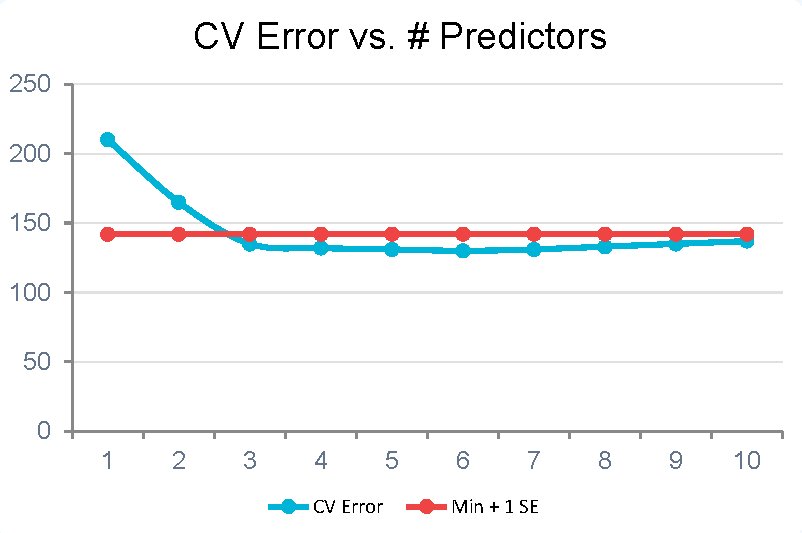
\includegraphics[width=\textwidth]{figures/varsel/varsel_cv_error_one_se.pdf}
\end{column}
\begin{column}{0.42\textwidth}
\scriptsize
\begin{block}{Rule:}
Select the SMALLEST model whose estimated test error is within 1 standard error of the lowest point on the curve.
\end{block}
\begin{block}{Rationale:}
If models look roughly equivalent, choose the simplest (fewest predictors).
\end{block}
\begin{exampleblock}{Credit data result:}
1-SE rule selects 3-variable model, even though 6-variable has lowest CV error.
\end{exampleblock}
\end{column}
\end{columns}
\end{frame}

% =====================================================================
\section{Part 3: Shrinkage Methods}

\begin{frame}
\centering
{\Large\usebeamercolor[fg]{structure}\textbf{Part 3: Shrinkage Methods}}

\vspace{12pt}
Constrain coefficient estimates toward zero to reduce variance
\end{frame}

% ---------------------------------------------------------------------
\begin{frame}{Shrinkage Methods: Core Idea}
\emph{\small Instead of selecting a subset, fit a model using ALL $p$ predictors --- but constrain the coefficient estimates.}

\textbf{Least Squares $\rightarrow$ Minimize:}
$$\mathrm{RSS} = \sum_{i=1}^n \Big(y_i - \beta_0 - \sum_j \beta_j x_{ij}\Big)^2$$

\textbf{Shrinkage $\rightarrow$ Minimize RSS + Penalty on $\beta$:}

\begin{columns}[T]
\begin{column}{0.49\textwidth}
\begin{block}{\small Ridge Regression}
\footnotesize
$\mathrm{RSS} + \lambda\cdot\sum_j \beta_j^2 \qquad (\ell_2 \text{ penalty})$

\vspace{4pt}
Shrinks all coeff toward 0; none set exactly to 0
\end{block}
\end{column}
\begin{column}{0.49\textwidth}
\begin{exampleblock}{\small The Lasso}
\footnotesize
$\mathrm{RSS} + \lambda\cdot\sum_j |\beta_j| \qquad (\ell_1 \text{ penalty})$

\vspace{4pt}
Shrinks coeff toward 0; some set EXACTLY to 0 $\rightarrow$ variable selection
\end{exampleblock}
\end{column}
\end{columns}
\end{frame}

% ---------------------------------------------------------------------
\begin{frame}{Ridge Regression}
{\small$$\min_{\beta}\bigg\{\sum_i \Big(y_i - \beta_0 - \sum_j \beta_j x_{ij}\Big)^2 + \underbrace{\lambda\cdot\sum_j \beta_j^2}_{\text{shrinkage penalty}}\bigg\}$$}

\scriptsize
\begin{tabular}{@{}>{\bfseries}p{0.12\textwidth}p{0.32\textwidth}|>{\bfseries}p{0.12\textwidth}p{0.32\textwidth}@{}}
\toprule
$\lambda = 0$ & Penalty disappears $\rightarrow$ identical to ordinary least squares. High variance, no bias.
& $\lambda \rightarrow \infty$ & All coefficients shrink to zero $\rightarrow$ null model (predicts mean). High bias, zero variance.\\
\midrule
Optimal $\lambda$ & Intermediate $\lambda$ balances bias-variance tradeoff. Chosen via cross-validation.
& Standard\-ize! & Predictors must be standardized before ridge regression --- penalties depend on variable scale.\\
\midrule
Intercept $\beta_0$ & The intercept is NOT penalized --- we only shrink $\beta_1, \ldots, \beta_p$ toward zero.
& All $p$ vars & Ridge keeps all $p$ predictors --- shrinks toward zero but never exactly to zero.\\
\bottomrule
\end{tabular}
\end{frame}

% ---------------------------------------------------------------------
\begin{frame}{Ridge: Bias-Variance Tradeoff}
\emph{As $\lambda$ increases: flexibility decreases $\rightarrow$ variance decreases, bias increases.}

\begin{columns}[T]
\begin{column}{0.56\textwidth}
\centering
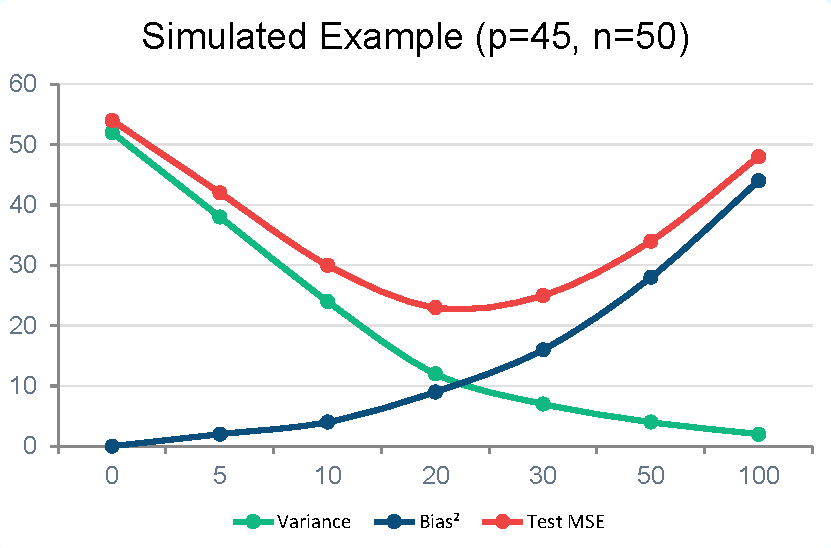
\includegraphics[width=\textwidth]{figures/varsel/varsel_ridge_bias_variance.pdf}
\end{column}
\begin{column}{0.42\textwidth}
\footnotesize
\begin{exampleblock}{Variance (Green)}
Decreases rapidly as $\lambda$ increases. Small $\lambda$ = high variance.
\end{exampleblock}
\begin{block}{Bias$^2$ (Blue)}
Near 0 when $\lambda=0$ (OLS). Rises as coefficients are forced toward 0.
\end{block}
\begin{alertblock}{Test MSE (Red)}
= Variance + Bias$^2$. Minimized at intermediate $\lambda \approx 20$ in this example.
\end{alertblock}
\end{column}
\end{columns}
\end{frame}

% ---------------------------------------------------------------------
\begin{frame}{The Lasso}
{\small$$\min_{\beta}\bigg\{\sum_i \Big(y_i - \beta_0 - \sum_j \beta_j x_{ij}\Big)^2 + \underbrace{\lambda\cdot\sum_j |\beta_j|}_{\ell_1 \text{ penalty}}\bigg\}$$}

\vspace{-6pt}
\textbf{Key Properties}
\vspace{-6pt}
\begin{columns}[T]
\begin{column}{0.49\textwidth}
\scriptsize
\begin{exampleblock}{Automatic Variable Selection}
The $\ell_1$ penalty forces some coefficients to EXACTLY zero $\rightarrow$ sparse models, like best subset selection.
\end{exampleblock}
\begin{block}{Sparse Models}
When $\lambda$ is sufficiently large, many $\beta_j = 0$. Only `signal' variables retain non-zero coefficients.
\end{block}
\end{column}
\begin{column}{0.49\textwidth}
\scriptsize
\begin{block}{Interpretability}
Resulting models involve only a subset of predictors --- far easier to interpret than Ridge.
\end{block}
\begin{block}{Tuning Parameter $\lambda$}
$\lambda = 0$: same as OLS. $\lambda \rightarrow \infty$: all coefficients zero. Cross-validation selects optimal $\lambda$.
\end{block}
\end{column}
\end{columns}
\end{frame}

% ---------------------------------------------------------------------
\begin{frame}{Why Lasso Performs Variable Selection}
\emph{The geometry of the $\ell_1$ constraint causes coefficients to hit zero --- $\ell_2$ does not.}

\begin{columns}[T]
\begin{column}{0.49\textwidth}
\begin{exampleblock}{\small Lasso ($\ell_1$) Constraint --- $|\beta_1| + |\beta_2| \le s$}
\footnotesize
Diamond shape --- has CORNERS at each axis.\\
Ellipses from OLS contours hit the corner $\rightarrow$ coefficient $= 0$ $\rightarrow$ variable excluded.
\end{exampleblock}
\end{column}
\begin{column}{0.49\textwidth}
\begin{block}{\small Ridge ($\ell_2$) Constraint --- $\beta_1^2 + \beta_2^2 \le s$}
\footnotesize
Circular shape --- NO corners.\\
Ellipses intersect the circle at a generic point $\rightarrow$ coefficients are non-zero (just small).
\end{block}
\end{column}
\end{columns}

\vspace{12pt}
{\small\emph{In higher dimensions ($p > 2$): Lasso constraint = polytope (sharp edges) $\rightarrow$ sparse solutions.}}
\end{frame}

% ---------------------------------------------------------------------
\begin{frame}{Ridge vs. Lasso: Side-by-Side}
\begin{center}
\scriptsize
\begin{tabular}{lll}
\toprule
\textbf{Property} & \textbf{Ridge Regression} & \textbf{The Lasso}\\
\midrule
Penalty & $\lambda\cdot\sum\beta_j^2$ ($\ell_2$ norm) & $\lambda\cdot\sum|\beta_j|$ ($\ell_1$ norm)\\
Coefficients & Shrunk toward 0, never exactly 0 & Some set exactly to 0\\
Variable selection & No --- includes all $p$ predictors & Yes --- automatic selection\\
Constraint region & Smooth circle (no corners) & Diamond with corners\\
Interpretability & Lower (all vars retained) & Higher (sparse model)\\
Best when\ldots & Many predictors, all with similar effect & Few true signal predictors\\
Prediction accuracy & Better when all $\beta \neq 0$ & Better when many $\beta = 0$\\
Shrinkage type & Proportional shrinkage & Soft-thresholding\\
\bottomrule
\end{tabular}
\end{center}

\centering
{\footnotesize\emph{Cross-validation determines which method works better on a given dataset.}}
\end{frame}

% ---------------------------------------------------------------------
\begin{frame}{Shrinkage Mechanics: A Simple Special Case}
\emph{When $X$ is diagonal ($n = p$), the shrinkage formulas have explicit, intuitive solutions.}

\begin{columns}[T]
\begin{column}{0.49\textwidth}
\begin{block}{\small Ridge Regression}
\footnotesize
$$\hat{\beta}^R_j = \frac{y_j}{1 + \lambda}$$
Each coefficient is simply scaled down by factor $1/(1+\lambda)$. All coefficients shrunk proportionally --- none reach zero.
\end{block}
\end{column}
\begin{column}{0.49\textwidth}
\begin{exampleblock}{\small The Lasso}
\footnotesize
$$\hat{\beta}^L_j = \mathrm{sign}(y_j)\cdot\max\left(|y_j| - \lambda/2,\, 0\right)\hspace{-6pt}$$
Coefficients with $|y_j| \le \lambda/2$ are set exactly to zero. Others are shrunk by a constant $\lambda/2$. This is SOFT-THRESHOLDING.
\end{exampleblock}
\end{column}
\end{columns}

\vspace{6pt}
{\footnotesize\emph{Key: Ridge shrinks ALL coefficients proportionally. Lasso shrinks by a fixed amount --- setting small ones to 0.}}
\end{frame}

% ---------------------------------------------------------------------
\begin{frame}{Bayesian Interpretation}
\emph{Ridge and Lasso emerge naturally from Bayesian regression with different priors on $\beta$.}

\begin{columns}[T]
\begin{column}{0.49\textwidth}
\begin{block}{\small Ridge Regression}
\footnotesize
\textbf{Gaussian prior on $\beta$}
$$p(\beta) \propto \exp\Big(-\lambda\cdot\sum\beta_j^2\Big)$$
Normal (Gaussian) distribution, flat at zero.

Ridge solution = Posterior MODE (and mean).

Expects: coefficients distributed randomly around zero.
\end{block}
\end{column}
\begin{column}{0.49\textwidth}
\begin{exampleblock}{\small The Lasso}
\footnotesize
\textbf{Double-Exponential (Laplace) prior on $\beta$}
$$p(\beta) \propto \exp\Big(-\lambda\cdot\sum|\beta_j|\Big)$$
Laplace distribution --- steeply peaked at zero.

Lasso solution = Posterior MODE only.

Expects: many coefficients are EXACTLY zero a priori.
\end{exampleblock}
\end{column}
\end{columns}

\vspace{4pt}
{\scriptsize\emph{Both methods assume: linear model + normal errors + simple $\beta$ prior $\rightarrow$ leads to penalized likelihood estimation.}}
\end{frame}

% =====================================================================
\section{\texorpdfstring{Part 4: Selecting the Tuning Parameter $\lambda$}{Part 4: Selecting the Tuning Parameter lambda}}

\begin{frame}
\centering
{\Large\usebeamercolor[fg]{structure}\textbf{Part 4: Selecting the Tuning Parameter $\lambda$}}

\vspace{12pt}
Cross-validation for optimal regularization strength
\end{frame}

% ---------------------------------------------------------------------
\begin{frame}{Selecting $\lambda$ via Cross-Validation}
\emph{The tuning parameter $\lambda$ controls the strength of regularization --- must be chosen carefully.}

\footnotesize
\begin{enumerate}
	\item \textbf{Define a grid of $\lambda$ values}\\
	{\scriptsize Typically spanning from very small ($\approx$ OLS) to very large (null model), e.g.\ 0.001 to 10,000 on log scale.}
	\item \textbf{Compute cross-validation error}\\
	{\scriptsize For each $\lambda$ in the grid, compute $k$-fold CV error across all candidate models.}
	\item \textbf{Select optimal $\lambda$}\\
	{\scriptsize Choose the $\lambda$ that yields the smallest cross-validation error.}
	\item \textbf{Refit on full data}\\
	{\scriptsize Using the selected $\lambda$, refit the model on all available observations to get final coefficient estimates.}
\end{enumerate}

{\scriptsize \textbf{Credit Data Results:} Ridge: optimal $\lambda$ is small (near OLS) --- mild shrinkage only. \ $|$ \ Lasso: finds correct 2 signal vars out of 45 in simulated example.}
\end{frame}

% ---------------------------------------------------------------------
\begin{frame}{Practical Guide: When to Use Which Method}
\small
\begin{tabular}{@{}p{0.47\textwidth}|p{0.47\textwidth}@{}}
\toprule
\textbf{$p$ is small ($< 40$)} & \textbf{$p$ is large ($\geq 40$) or $n < p$}\\
\emph{Best Subset $\cdot$ Forward/Backward Stepwise} & \emph{Forward Stepwise $\cdot$ Ridge Regression $\cdot$ Lasso}\\
\midrule
\textbf{Many predictors, all roughly equally important} & \textbf{Few true signal predictors (sparse model expected)}\\
\emph{Ridge Regression} & \emph{Lasso}\\
\midrule
\textbf{Model interpretability is critical} & \textbf{Unsure which method works best}\\
\emph{Lasso $\cdot$ Best Subset} & \emph{Use cross-validation to compare $\cdot$ Both Ridge and Lasso $\cdot$ Evaluate on validation data}\\
\bottomrule
\end{tabular}
\end{frame}

% ---------------------------------------------------------------------
\begin{frame}{Key Takeaways}
\begin{columns}[T]
\begin{column}{0.49\textwidth}
\scriptsize
\begin{enumerate}
	\item \textbf{RSS/$R^2$ are insufficient}\\
	They always improve with more predictors --- use test error estimates ($C_p$, BIC, adjusted $R^2$, CV) instead.
	\item \textbf{Best Subset is thorough but slow}\\
	Computationally infeasible for $p > 40$. Forward/backward stepwise offer efficient alternatives with $O(p^2)$ models.
	\item \textbf{Cross-validation is king}\\
	Provides direct, assumption-free test error estimates. The one-standard-error rule favors simpler models when errors are similar.
\end{enumerate}
\end{column}
\begin{column}{0.49\textwidth}
\scriptsize
\begin{enumerate}
	\setcounter{enumi}{3}
	\item \textbf{Ridge reduces variance}\\
	By shrinking coefficients toward zero --- best when all predictors are weakly related to the response.
	\item \textbf{Lasso selects variables}\\
	$\ell_1$ penalty forces exact zeros --- best when only a few predictors truly matter. Interpretable sparse models.
	\item \textbf{No universal winner}\\
	Neither Ridge nor Lasso always dominates. Cross-validate to determine which works best for your data.
\end{enumerate}
\end{column}
\end{columns}

\centering
{\tiny\emph{Based on: James, Witten, Hastie \& Tibshirani --- An Introduction to Statistical Learning, Chapter 6}}
\end{frame}

\end{document}
